\newcommand{\JastAdd}{\textsc{Jast\-Add}}
\newcommand{\ExtendJ}{\textsc{ExtendJ}}
\newcommand{\IntraJ}{\textsc{IntraJ}}
\newcommand{\CAT}{\textsc{CAT}}
\newcommand{\eval}[2]{\textsc{#1}$_{\color{gray!70}{\pm#2}}$}
\newcommand{\basicStacked}{\textsc{Basic\-Stacked}}
\newcommand{\relaxedMonolithic}{\textsc{Relaxed\-Monolithic}}
\newcommand{\relaxedstacked}{\textsc{Relaxed\-Stacked}}
\newcommand{\relmon}{\textsc{rm}} %Abbreviation for relaxed Monolithic
\newcommand{\relstk}{\textsc{rs}} %Abbreviation for relaxed stacked
\newcommand{\code}[1]{\texttt{#1}}
\newcommand{\slowdown}[1]{$-$ #1 \color{red}{$\downarrow$}}
\newcommand{\speedup}[1]{$+$ #1 \color{teal}{$\uparrow$}}
\newcommand{\slowdownnew}[1]{$\times$ #1 \color{red}{$\downarrow$}}
\newcommand{\speedupnew}[1]{$\times$ #1 \color{teal}{$\uparrow$}}
\newcommand{\evaltimeout}[1]{%
    $\geq$ \textsc{#1}~\raisebox{-0.2\height}{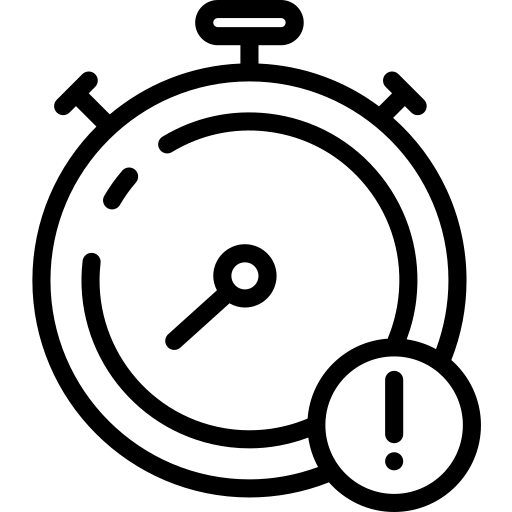
\includegraphics[height=1em]{timeout.png}}%
}
\newcommand{\gespeedup}[1]{$\geq$ #1 \color{teal}{$\uparrow$}}
\newcommand{\same}{\color{gray}{$\approx$}}

\newcommand{\extendjbaseline}{\ExtendJ$_{\relmon}$}
\newcommand{\extendjrelaxed}{\ExtendJ$_{\relstk}$}



\newcommand{\intrajbaseline}{\IntraJ$_{\relmon}$}
\newcommand{\intrajrelaxed}{\IntraJ$_{\relstk}$}


\newcommand{\percentwrt}[1]{\footnotesize
$\Delta$\%$^{\scriptscriptstyle\text{w.r.t}}_{\scriptscriptstyle\text{#1}}$%
}











\lstset{basicstyle=\scriptsize\ttfamily,
        escapeinside={/+}{+/},
        keywordstyle=[1]\bfseries}
